%Dave's handout 1.7 intro 2nd derivatives
%Dave's handout 2.2 2nd derivative rule
\vspace{-0.25 in}
\begin{framed}
\subsection*{Objectives}
\begin{itemize}
    \item Apply the \textbf{Chain Rule} and the product/quotient rules correctly in combination when both are necessary.
    \item Be able to apply the concept of the \emph{Chain Rule} to \textbf{related rates} application.
\end{itemize}

%%%Reading Assignment%%%
\subsection*{Suggested Reading:}
\begin{itemize}
\item \cite{openstax}\footnotemark[1]\textsuperscript{,}\footnotemark[2]
    \begin{itemize}
        \item Section 3.6 The Chain Rule

    \end{itemize}
\item \cite{Calaway}\footnotemark[3]
   \begin{itemize}
         \item Section 2.11 Implicit Differentiation and Related Rates
        \begin{itemize}
            \item Only Examples 3-4.
        \end{itemize}
        
    \end{itemize}


\end{itemize}
%\subsection*{Supplemental Materials:}
%%%Key Terms%%%
\subsection*{Key Terms and Concepts:} 

\begin{multicols}{2}
\begin{itemize}
    \item The Chain and Power Rules combined
    \item The Chain and Product Rules combined
    \item The Chain and Quotient Rules combined
    \item Related Rates
\end{itemize}
\end{multicols}
\end{framed}
\footnotetext[1]{Available free to download from \url{https://openstax.org/details/books/calculus-volume-1} .}
\footnotetext[2]{Disregard any examples with trigonometry.}
\footnotetext[3]{Available free to download from \url{http://www.opentextbookstore.com/details.php?id=14} .}


\newpage
%%%%%%%%%%START LESSON CONTENT%%%%%%%%%%%%%
%\noindent\makebox[\linewidth]{\rule{\textwidth}{0.8pt}}
\Opensolutionfile{ans}[ans11]
\Opensolutionfile{ansL}[ansL11]
%%%%%%%%%%%%%%%%Start First Topic%%%%%%%%%%%%%%%%%%%%%%%%%%%%%
\noindent The Chain Rule was introduced in lesson \ref{GenPower} using the prime notation. You have learned how to use the Chain Rule with the Power Rule. The combination of the two rules is so called the General Power Rule. In lesson \ref{rateChange}, the \emph{Leibniz} notation was introduced to help with the intuition of the Chain Rule. In this lesson, we will learn how to use the \textbf{Chain Rule} in a more complex way----with the \textbf{Product Rule} and with the \textbf{Quotient Rule}.
 %%%%%%%%%%%% The Chain Rule Box %%%%%%%%%%%%%
\begin{tcolorbox}[title = {Review: The Chain Rule}]

\noindent Let $f(x)$ and $g(x)$ be functions. For all $x$ in the domain of $g$ for which $g$ is differentiable at $x$ and $f$ is differentiable at $g(x)$, the derivative of the \emph{composite function} \\
\begin{equation}
    h(x)=(f\circ g)(x)=f(g(x))
\end{equation}
is given by
\begin{equation}\label{eq:MoreChainRule}
    h'(x)=f'(g(x))\cdot g'(x)
\end{equation}
\noindent In other words, the derivative of a composition of a function (denoted as \((f\circ g)'(x)\) is the derivative of the outside function $f$ (with respect to the original inside function) \emph{times} the derivative of the inside function $g$.\\

For $h(x)=f(g(x))$, let $u=g(x)$ and $y=h(x)=f(u)$. Using the \emph{Leibniz} notation form, the $h'(x)$ can be written as follows:\\
\begin{equation}\label{eq:LeibnizChain}
    \displaystyle\frac{dy}{dx}=\frac{dy}{du}\cdot \frac{du}{dx}
\end{equation}
\end{tcolorbox}
\subsection*{Review: The Chain and Power Rules Combined}
%%%Adapt from Example 3.54 from OpenStax;Calculus I;3.6 Chain Rule%%%
\begin{example}\label{exMoreChain1}
Given $h(x)=(2x+1)^5$,   
\renewcommand{\labelenumi}{\textbf{(\alph{enumi})}}
\begin{enumerate}[leftmargin=*]
    \item Find the derivative of $h(x)$ using the \textbf{Chain Rule} with the \underline{prime notation form} in equation \ref{eq:MoreChainRule}.\newpage
    \item Find the derivative of $h(x)$ using the \textbf{Chain Rule} with the \underline{\emph{Leibniz} notation form} in equation \ref{eq:LeibnizChain}.\vspace*{\stretch{1}}
\end{enumerate}
    %%short answer
    \begin{sol}
    \onehalfspacing{
    \begin{enumInline1}
    \item $h'(x)=10(2x+1)^4$
    \item $\displaystyle\frac{dy}{dx}=10(2x+1)^4$
    \end{enumInline1} }
    \end{sol}
    %%solution
    \begin{solL}
    Complete solution here.....
    
    \end{solL}
    
\end{example}

%%%%%%%%%%%%%%%The Chain and Product Rules Combined%%%%%%%%%%%%
\subsection*{The Chain and Product Rules Combined}
%%%Example 3.54 from OpenStax;Calculus I;3.6 Chain Rule%%%
\begin{example}
Given $h(x)=(2x+1)^5(3x-2)^7$, find the derivative of $h(x)$ using the \textbf{Chain Rule} with the \underline{prime notation form} in equation \ref{eq:MoreChainRule}.\vspace*{\stretch{1}}

    %%short answer
    \begin{sol}
    $h'(x)=(2x+1)^4(3x-2)^6(72x+1)$
    \end{sol}
    %%solution
    \begin{solL}
    Complete solution here.....
    
    \end{solL}
    
\end{example}
\newpage
%%%%%%%%%%%%%%%%The Chain and Quotient Rules Combined%%%%%%%%%%%%
\subsection*{The Chain and Quotient Rules Combined}
%%%CheckPoint 3.37 from OpenStax;Calculus I;3.6 Chain Rule%%%
\begin{example}
Given $h(x)=\displaystyle\frac{x}{(2x+3)^3}$, find the derivative of $h(x)$ using the \textbf{Chain Rule} with the \underline{prime notation form} in equation \ref{eq:MoreChainRule}.\vspace*{\stretch{1}}

    %%short answer
    \begin{sol}
    $h'(x)=\displaystyle\frac{3-4x}{(2x+3)^4}$
    \end{sol}
    %%solution
    \begin{solL}
    Complete solution here.....
    
    \end{solL}
    
\end{example}

%%%Example 3.58 from OpenStax;Calculus I;3.6 Chain Rule%%%
\begin{example}
Given $h(x)=\left(\displaystyle\frac{x}{3x+2}\right)^5$, find the derivative of $h(x)$ using the \textbf{Chain Rule} with the \underline{\emph{Leibniz} notation form} in equation \ref{eq:LeibnizChain}.\vspace*{\stretch{1}}
    %%short answer
    \begin{sol}
    $\displaystyle\frac{dy}{dx}=\frac{10x^4}{(3x+2)^6}$
    \end{sol}
    %%solution
    \begin{solL}
    Complete solution here.....
    
    \end{solL}
    
\end{example}
\newpage
\subsection*{Application Using The Chain Rule: Related Rates}
%%%From the "Related Rates" box in Applied Calculus by Calaway;Chapter 2 section 11 Implicit Differentiation and Related Rates%%%
\begin{tcolorbox}[title = {Strategy for Finding Related Rates}]
When working with a related rates problem,
\begin{enumerate}
    \item Identify the quantities that are changing, and assign them variables.
    \item Find an equation that relates those quantities.
    \item Differentiate both sides of that equation with respect to time.
    \item Plug in any known values for the variables or rates of change.
    \item Solve for the desired rate.
\end{enumerate}
\end{tcolorbox}
%%%Example 3 from Applied Calculus by Calaway;Chapter 2 section 11 Implicit Differentiation and Related Rates%%%

\begin{wrapfigure}[7]{r}{0.35\textwidth}
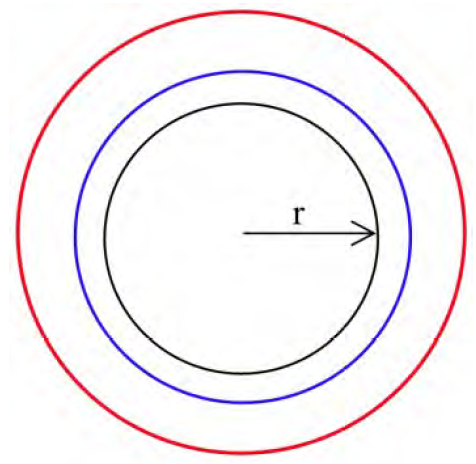
\includegraphics[width=0.7\textwidth]{chainRule/exTownBorder.png}
\end{wrapfigure}
\hfill \break
\vspace{-0.5in}
\begin{example}
Suppose the border of a town is roughly circular, and the radius of that circle has been increasing at a rate of 0.1 miles each year. 
\renewcommand{\labelenumi}{\textbf{(\alph{enumi})}}
\begin{enumerate}[leftmargin=*]
    \item Determine the equation that gives the relationship between the \textbf{town area} (in mile\raise0.75ex\hbox{\scriptsize{2}}) , $\bm{A}$ and the town radius (in mile), $\bm{r}$. \emph{Include the appropriate unit.} \vspace*{\stretch{1.5}}
\end{enumerate}

\renewcommand{\labelenumi}{\textbf{(\alph{enumi})}}
\begin{enumerate}[leftmargin=*]
    \setcounter{enumi}{1}
    \item Determine the equation that gives the relationship between the \textbf{town radius} , $\bm{r}$ and the time (in year), $\bm{t}$. \emph{Include the appropriate unit.}\vspace*{\stretch{1}}
    \newpage
    \item Using the \textbf{Chain Rule} with the \underline{\emph{Leibniz} notation form} in equation \ref{eq:LeibnizChain}, determine the \textbf{related rates equation} that gives the relationship between the rate of change of the circumference of the town border, $\displaystyle\frac{dC}{dt}$ and the rate of change of the radius of the town border, $\displaystyle\frac{dr}{dt}$. \emph{Include the appropriate unit.}\vspace*{\stretch{4}}
    \item Find \textbf{how fast the area} of the town has been increasing when the radius is 5 miles. \emph{Include the appropriate unit.} \vspace*{\stretch{1}}
    
\end{enumerate}
    %%short answer
    \begin{sol}
    \onehalfspacing{
    \begin{enumInline1}
    \item $A(r)=\pi r^2$ mile\raise0.75ex\hbox{\scriptsize{2}} 
    \item $r(t)=0.1t$ mile per year
    \item $\displaystyle\frac{dA}{dt}=2\pi r\displaystyle\frac{dr}{dt}$ mile\raise0.75ex\hbox{\scriptsize{2}}
    \item Around 3.14 mile\raise0.75ex\hbox{\scriptsize{2}} per year
    \end{enumInline1} }
    \end{sol}
    %%solution
    \begin{solL}
    Complete solution here.....
    
    \end{solL}
    
\end{example}

%%%%%%%%%%%%%%%End Lesson%%%%%%%%%%%%%%%%%%
\Closesolutionfile{ans}
\Closesolutionfile{ansL}

%%%Short Answers to Examples%%%
\vspace*{\fill}

\subsection*{Short Answers to Examples}
%\vspace{-0.25cm}
%\begin{multicols}{2}
\input{ans11}
%\end{multicols}


